\section{Model}

\subsection{Data}
\frame
{
\frametitle{Data}
\begin{block}{}
Sandia has provided MD simulation results which we will use as training data for our ML models. We also have a set of Python scripts to help us process and load the data into certain data structures/models that we create.
\end{block}
}

\frame
{
\frametitle{Features}
\begin{block}{}
Data includes features such as:
\begin{itemize}
    \item $x, y, z$ coordinates for each atom
    \item charge
    \item stress tensor
    \item bond connectivity
    \item newly formed/broken bonds
    \item $SiO_n$ distribution
    \item $Q_n$ distribution
    \item $nuc_v$
\end{itemize}
\end{block}
}

\frame
{
  \frametitle{Example of Data}
  \begin{block}{}

			\begin{figure}[h]
				\centering
				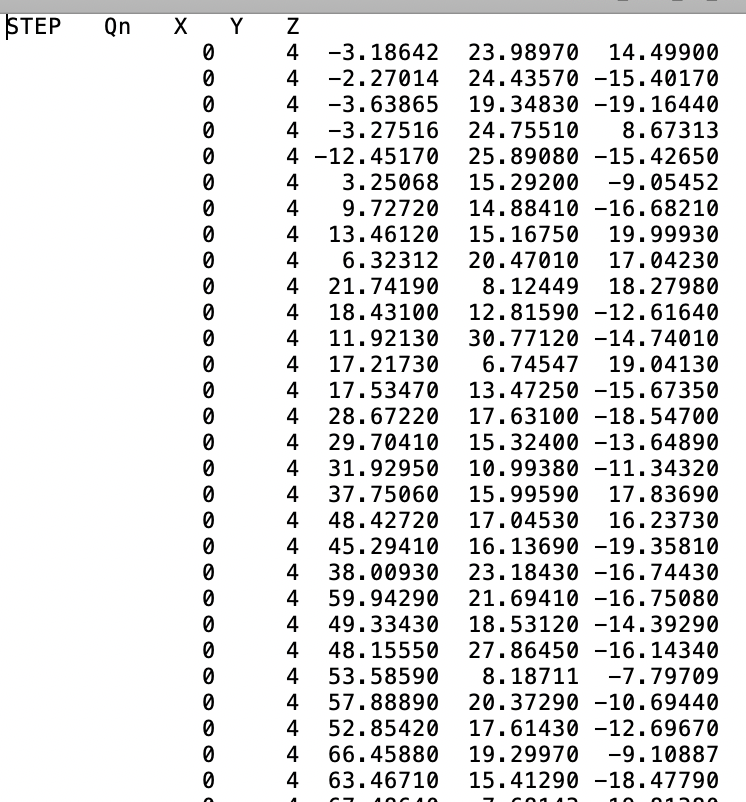
\includegraphics[width=.5\textwidth]{Q_n.png}
			\end{figure}
 
    \end{block}
}


\frame{
\frametitle{Methods}
\begin{block}

Give an overview of what our methods are:
\begin{itemize}
    \item Graph Representations
    \item Ground Truth
    \item Feature Description
    \item Machine Learning Methods
\end{itemize}
\end{block}
}

%%%%%%%%%%%%%%%%%%%%%%%%%%%%%%%%%%%

\subsection{Graph Representations}

\begin{frame}[t]{Graph Representations}
The graph, denoted as $G(t)=\{V(t),E(t)\}$, has the following three topology representations. $V(t)$ and $G(t)$ represent the set of vertices and edges at time t, respectively.

 \begin{columns}[t]
 
   \column{0.3\textwidth}
   \begin{block}{Basic Graph}
   \begin{itemize}
   \begin{footnotesize}
       \item V: Si, O atoms
       \item E: Chemical bond between atoms
    \end{footnotesize}
    \end{itemize}
    \begin{figure}
	    \centering
        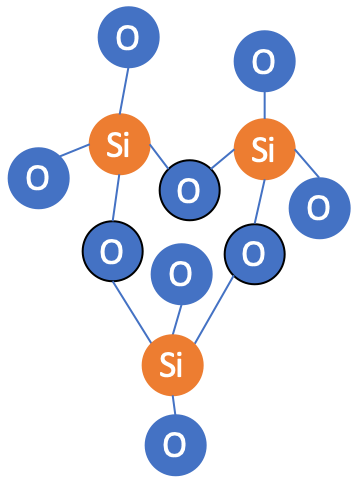
\includegraphics[width=.5\textwidth]{images/basic.png}
	\end{figure}
   \end{block}
   
   \column{0.3\textwidth}
   \begin{block}{Reduced Graph}
   \begin{itemize}
   \begin{footnotesize}
       \item V: Si atoms
       \item E: Bridging Oxygens
    \end{footnotesize}
   \end{itemize}
    \begin{figure}
	    \centering
        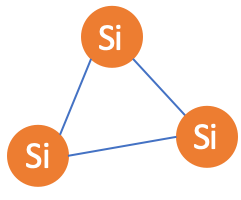
\includegraphics[width=.5\textwidth]{images/reduced.png}
	\end{figure}
   \end{block}
   
   \column{0.3\textwidth}
   \begin{block}{Topological Graph}
   \begin{itemize}
   \begin{footnotesize}
       \item V: Rings(closed paths)
       \item E: Bridging oxygen
    \end{footnotesize}
   \end{itemize}
    \begin{figure}
	    \centering
        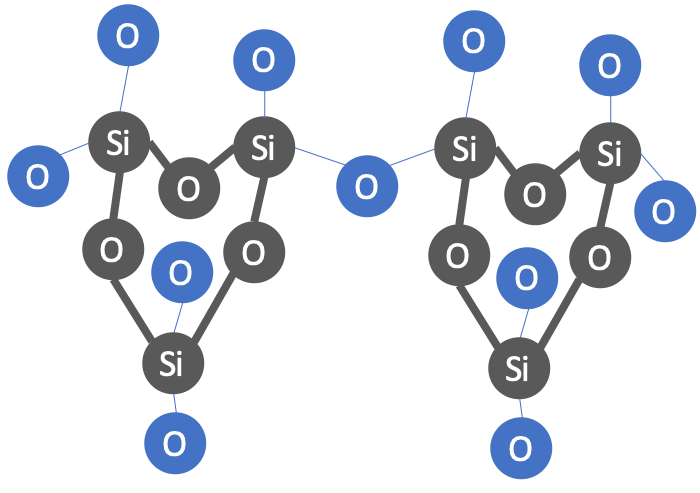
\includegraphics[width=.5\textwidth]{images/ring.png}
	\end{figure}   
   
   
   \end{block}
   
 \end{columns}
\end{frame}

\begin{frame}
\frametitle{Ground Truth}

\begin{minipage}[0.2\textheight]{\textwidth}
\begin{columns}[T]
    \begin{column}{0.5\textwidth}
    
    \begin{itemize}
    \begin{footnotesize}
    \item The ground truth is defined as whether or not an atom is part of a fracture at a certain time step. Thus, $\textbf{y} \in \{0, 1\}^n$, where $n$ is the total number of atoms.
    \item As the figure shows, some atoms are not highlighted in red, though they are on the fracture surface. So a K-nearest-neighbors algorithm will be applied to label those atoms.
    \end{footnotesize}  
    \end{itemize}
    \end{column}
    
    \begin{column}{0.5\textwidth}
    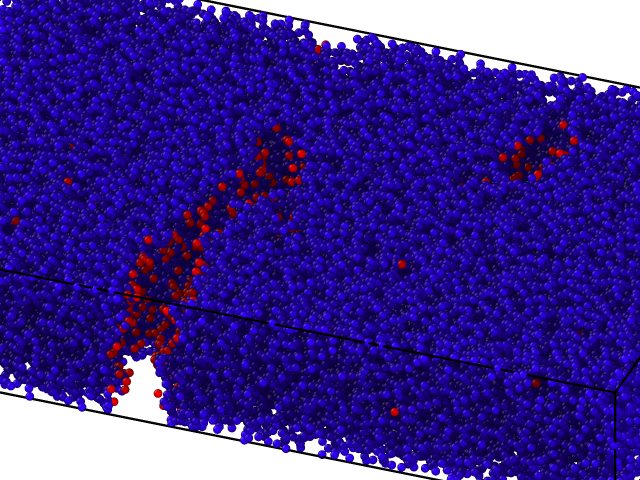
\includegraphics[width=5.5cm]{images/face.png}
    \end{column}
\end{columns}
\end{minipage}
\end{frame}

\frame{
\frametitle{Feature Description}
This slide is to talk about feature description
}




\subsection{Machine Learning Methods}
\frame{
\frametitle{Machine Learning Methods}
Talk about machine learning methods!! yayyyyy


}


\frame
{
\frametitle{Voronoi Cell Volume}
\begin{block}{}
We also define the ground truth using a local density measure that we call the \textbf{Voronoi cell volume, $v_i$}, around a certain atom $i$. It is the empty space surrounding an atom.
\newline\newline
If $v_i$ exceeds a certain threshold, then the atom $i$ is defined as part of a nucleation event. Thus, $y_i = 1$.
\newline\newline
The threshold:
\centering $nuc_v = \frac{(v_i - \mu_v)}{\sigma_v}$
Thus, the ground truth can be defined as:
    \[
    y_i = \begin{cases}
      0 & \text{if }(nuc_v)_i \le 1 \\
      1 & \text{if }(nuc_v)_i > 1 \\
    \end{cases} 
    \]
\end{block}
}

\frame
{
  \frametitle{Example of 3D Fracture}
  \begin{block}{}

\begin{figure}[h]
				\centering
				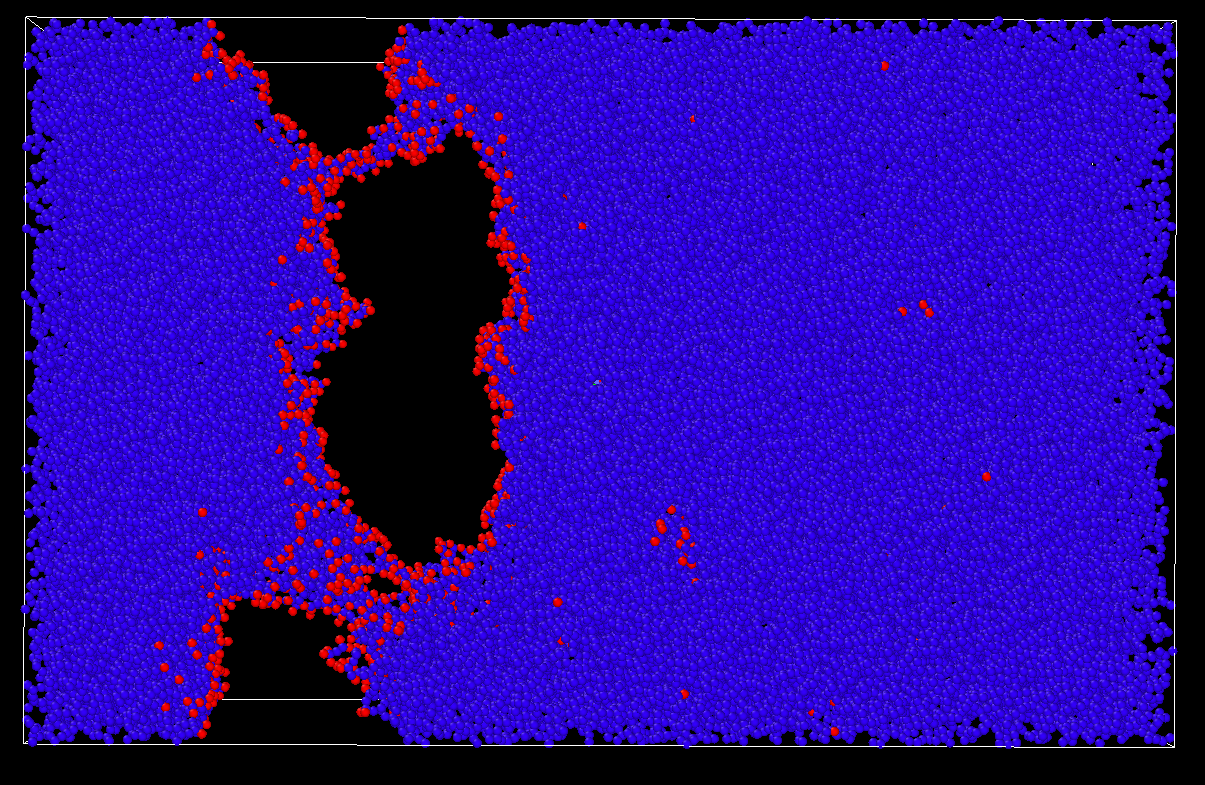
\includegraphics[width=.7\textwidth]{volcolor.png}
				 \caption{Red atoms have a surrounding volume greater than the threshold}
\end{figure}
 
    \end{block}
}